\subsection{Backpropagation}

Back propagation is a learning algorithm which aims to minimize the errors/cost function of the NN. Through this learning algorithm, the random weights and biases which were initially given to the network will be optimized to give the best output.

Output of each node is the sum of the multiplications of the output of previous nodes by certain weights. Therefore we can associate how much error is coming with every weight and how much error has been brought from each particular node from the previous layer.

To understand this better it is worth imagining the following example:
\begin{itemize}
   \item  node 1 in the output layer of the NN should be equal to 0.01
   \item  instead the NN is providing us with 0.8
\end{itemize}

In this case we should do the following:
\begin{enumerate}
   \item Calculate the error of the node (-0.79 in our example)
   \item Calculate how much error has been brought by every link to this node
\end{enumerate}

For instance if weight \(w_{11}\) is 0.6 and \(w_{21}\) is 0.4 then they are associated with an error of -0.79 multiplied by 0.6 and -0.79 multiplied by 0.4 respectively (see Figure \ref{fig:bp}).

\begin{figure}[H]
    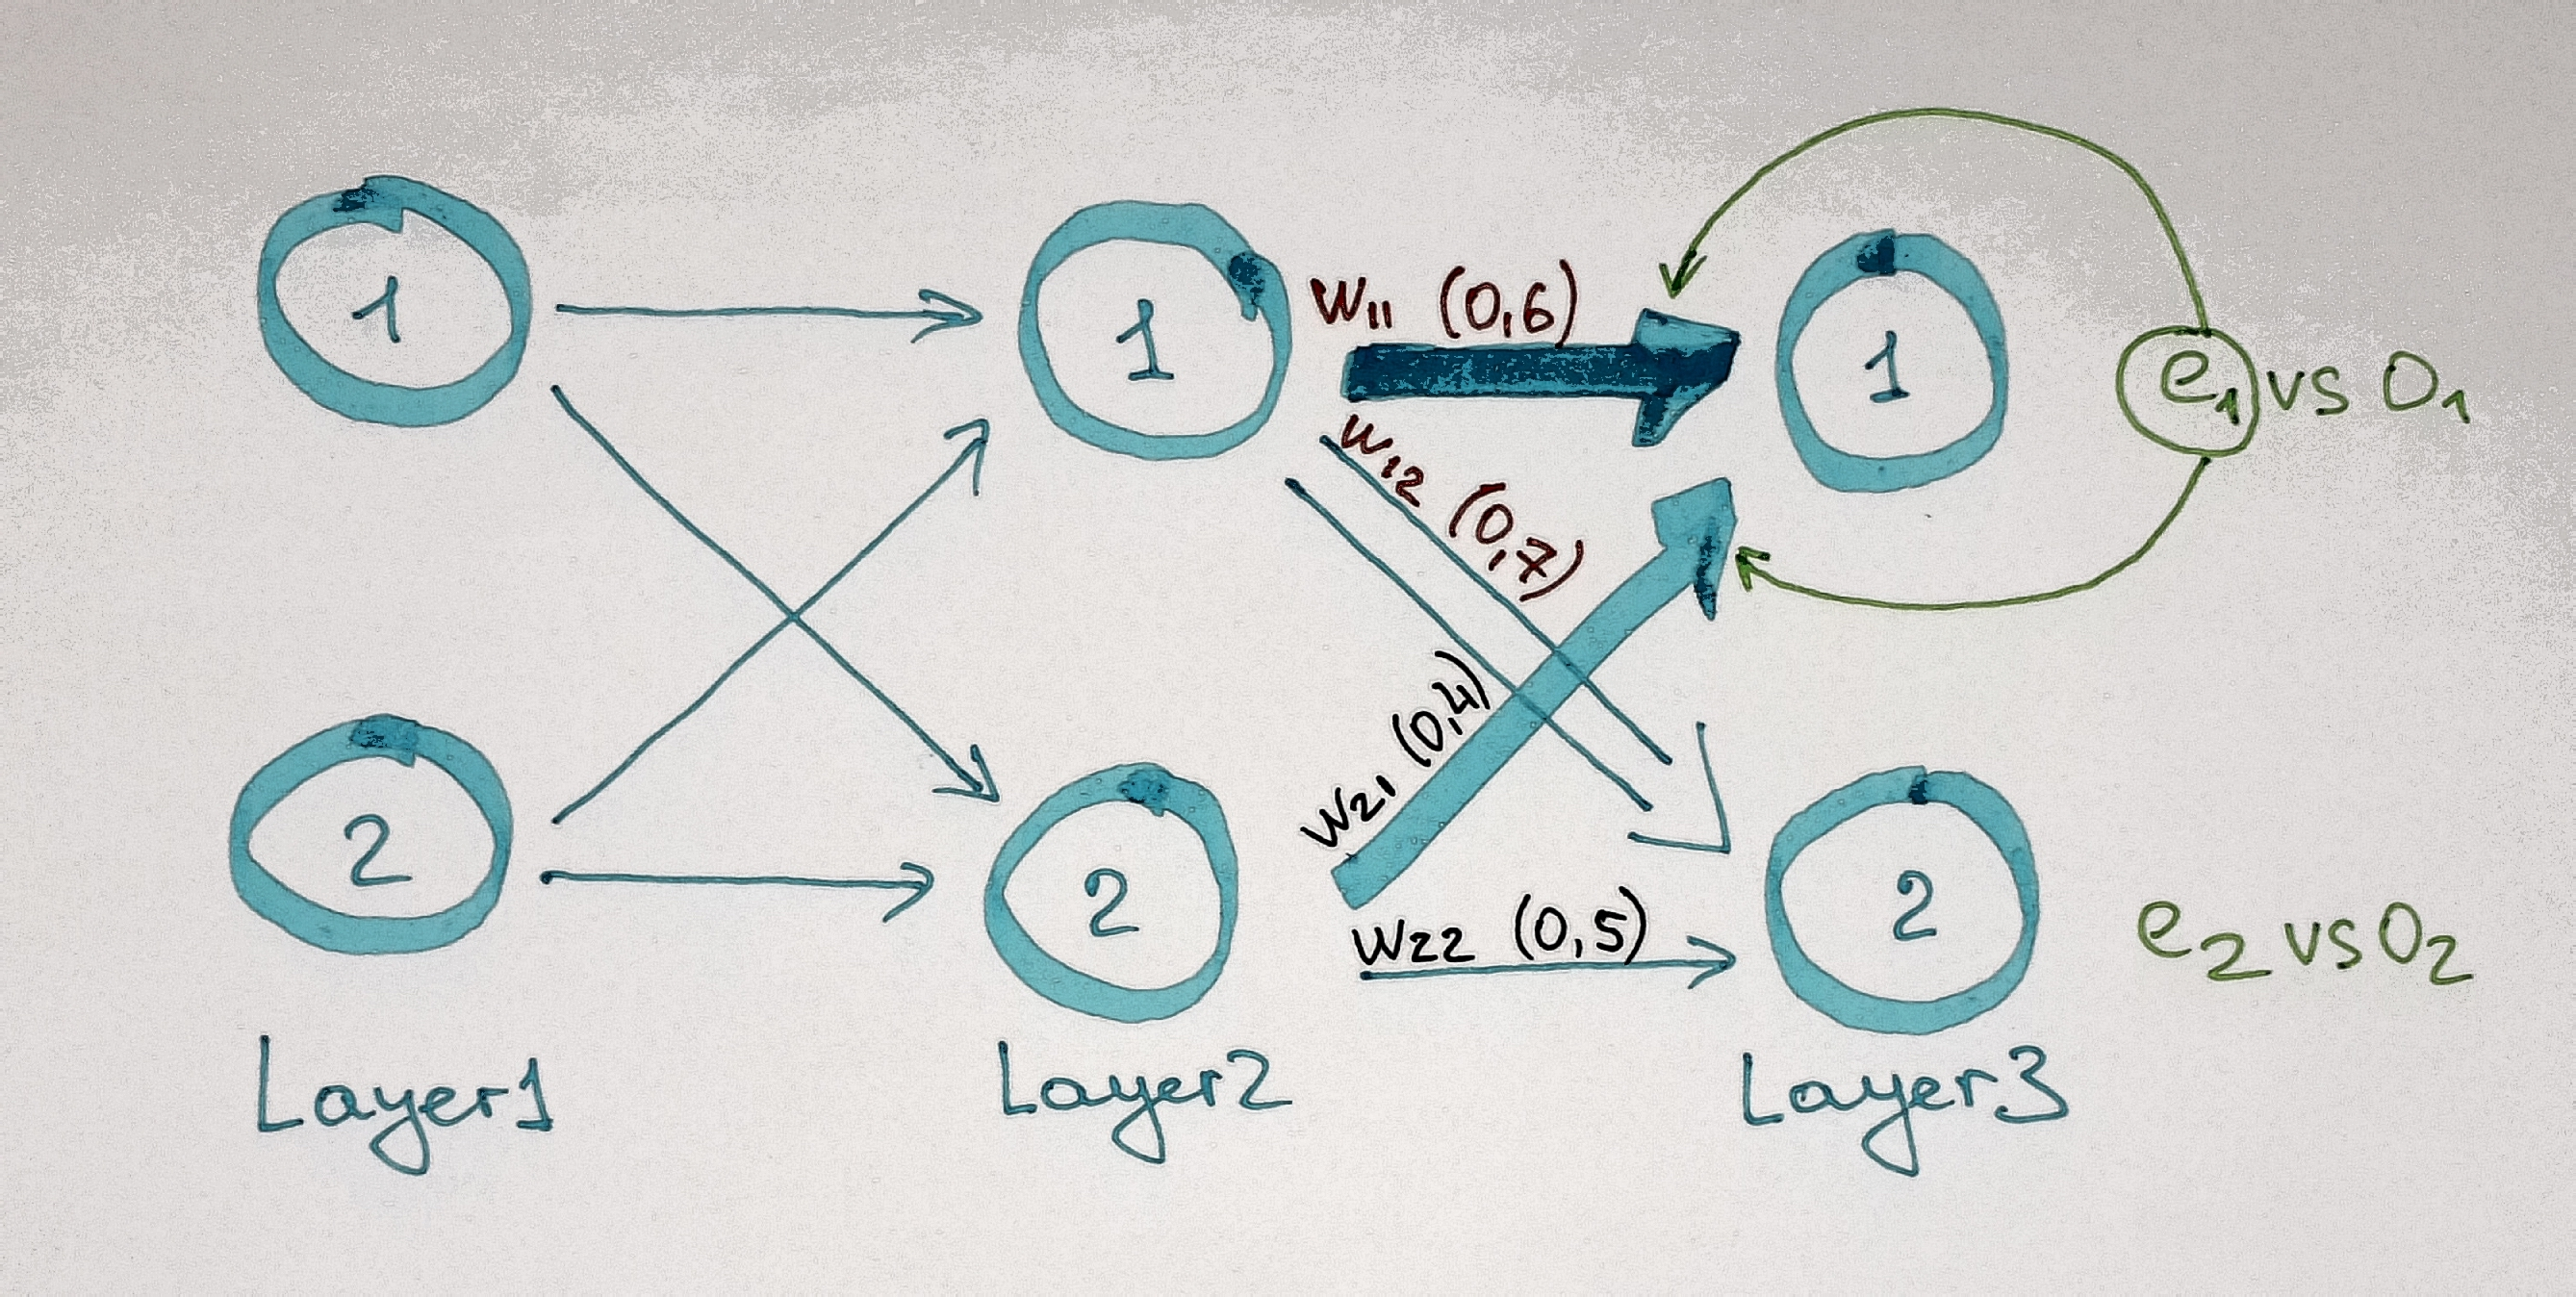
\includegraphics[width=\linewidth]{pics/bp.jpg}
    \caption{\label{fig:bp} Backpropagation}
\end{figure}

After calculation of how much error is associated with every weight we can obtain the errors for the nodes in the proceeding layer.
 
For instance error term for node 1 in the hidden layer will be equal to:
\begin{itemize}
   \item the sum of errors associated with all the weights (\(w_{11}\) and \(w_{12}\) in our case) that link this node with the next layer (see Figure \ref{fig:bp}).
\end{itemize}


Once we repeat this procedure for all the nodes in all layers we can find out how much every node should be changed.

To do so in Python we just need to make multiplication of vector that contain errors by corresponding matrix of weights.

\begin{lstlisting}[language=Python]
    Find the errors associated with hidden layer output:
    h_errors = np.dot(w_h_o.T, o_errors),
    h_errors[0:10] # errors in the hidden layer - show the first 10 nodes out of 90.
\end{lstlisting}

\begin{lstlisting}
    array([[ 0.39443768],
    [-0.16865836],
    [ 0.0304721 ],
    [-0.85442941],
    [-0.19828127],
    [-0.53651297],
    [ 0.52033741],
    [-0.2781908 ],
    [-0.07071894],
    [-1.63579796]])
\end{lstlisting}

\subsection{Gradient Descent}

Gradient descent is one the most popular algorithms to optimize the neural networks. The name gradient descent is rooted in the procedure where the gradient is repeatedly evaluated to update the parameters. The objective of the gradient descent is to find weight parameters that will minimize the cost function.

To understand the concept of gradient descent we should ask ourselves the following question: What can be done to improve the weights we have assigned randomly at the beginning, so that the overall result improves?

To change the output of any node we should change the weights that connect it with the previous layer. Basically we want to find out how much error in every node changes once we change associated weights. Next we want to select the weights that would lead to a minimal error in the output layer. That can be achieved by differentiation of the cost function and search for its minimum.

Given multidimensionality of the function, which we need to differentiate, the search for its minimum can be a complicated task. This task is similar to some extent to the search of the path in the darkness from the top of a mountain to its valley. Because it is dark it is almost impossible to reach the valley immediately. The only way to achieve the goal is by exploring the neighbourhood (the radius you are able to see) and tacking small steps in the direction that leads downhill and constantly updating the path for the next steps. This process is illustrated on the Figure \ref{fig:gradient-descent}:

\begin{figure}[H]
    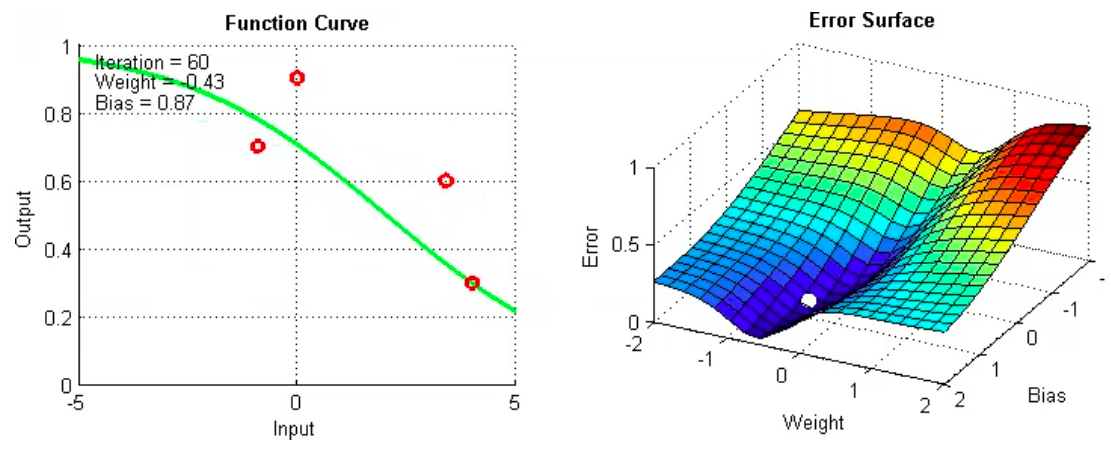
\includegraphics[width=\linewidth]{pics/gradient_descent.png}
    \caption{\label{fig:gradient-descent} How Gradient Descent works. Source: Giphy.com}
\end{figure}

Mathematically the differentiation process can be illustrated on the example of weights between output and hidden layers \(w_{ho}\). The same process but with corresponding values should be applied for the weights between input and hidden layers \(w_{ih}\).

As it can be seen from the formulas below the error we want to minimize \(E\) can be defined as the sum of squared differences between the target \(t_n\) and output \(o_n\) values of the NN. The sum of differences for all the nodes in the layer is relevant but when doing calculation for a particular node this sum can be omitted - only the difference between particular output \(o_o\) and target \(_o\) matters.

Target value is constant. Output value depends on weights and is obtained after applying sigmoid function to the sum of inputs (outputs of the previous layer - \(o_h\) multiplied by corresponding weights \(w_{ho}\).

\begin{equation}
\frac{\partial E}{\partial w_{ho}}=\frac{\partial}{\partial w_{ho}}\displaystyle\sum_{n=1}^{n} (t_n-o_n)^2=\frac{\partial}{\partial w_{ho}}(t_o-o_o)^2
\end{equation}

\begin{equation}
\frac{\partial E}{\partial w_{ho}}=\frac{\partial E}{\partial O_{o}}\frac{\partial O}{\partial w_{ho}}=-2(t_o-o_o)\frac{\partial O}{\partial w_{ho}}
\end{equation}

\begin{equation}
\frac{\partial E}{\partial w_{ho}}=-2(t_o-o_o)\frac{\partial}{\partial w_{ho}}sigmoid(\sum(w_{ho}o_h)
\end{equation}

The formula for derivative of the sigmoid function is formula 4. It is necessary to keep in mind that the sum to which we apply sigmoid function also depends on the change of weights \(w_{ho}\). Therefore one should follow the chain rule for derivation.

\begin{equation}
\frac{\partial}{\partial x}sigmoid(x)=sigmoid(x)(1-sigmoid(x))
\end{equation}

\begin{equation}
\frac{\partial E}{\partial w_{ho}}=-2(t_o-o_o)sigmoid(\sum_{h=1}^{h} (w_{ho}o_h)(1-sigmoid(\sum_{h=1}^{h} (w_{ho}o_h))\frac{\partial (\sum_{h=1}^{h} (w_{ho}o_h))}{\partial w_{ho}}
\end{equation}

\begin{equation}
\frac{\partial E}{\partial w_{ho}}=-2(t_o-o_o)sigmoid(\sum_{h=1}^{h} (w_{ho}o_h)(1-sigmoid(\sum_{h=1}^{h} (w_{ho}o_h))o_h
\end{equation}

The formula we derive is for one particular node. We can however apply it to all the nodes in the layer. In order to do so the only thing we need is to consider this formula in matrix notation. Thus, necessary update of weights linked to all the nodes in a layer will be calculated.

\begin{equation}
\frac{\partial E}{\partial W_{ho}}=-2*O_{error}*O_{output}*(1-O_{output})*O_h^T
\end{equation}

After solving the minimization problem we can update the weights we have assigned before.

\begin{equation}
new W_{ho}=old W_{ho}-\frac{\partial E}{\partial W_{ho}}
\end{equation}

\begin{equation}
\Delta W_{ho}=-2*(T_o-O_o)*sigmoid(O_o)*(1-sigmoid(O_o)*O_h^T
\end{equation}

In code this can be represented as follows:

\begin{lstlisting}[language=Python]
    # Update the matrix for weights between hidden and output layers:
    w_h_o += np.dot((o_errors * o_output * (1.0 - o_output)), np.transpose(h_output)) # 2 can be omitted as being related to the learning rate.
    # Update the matrix for weights between input and hidden layers:
    w_i_h += np.dot((h_errors * h_output * (1.0 - h_output)), np.transpose(input))"
\end{lstlisting}

\subsection{Learning Rate}

Now, there is something else, we should add in the weights updating procedure. If we completely change our weights with every new observation - our model learns to predict only the last input. Instead of updating weights 100 \% every time we can change them only partially - this way every new observation will bring some new knowledge while the previous one will still be in memory even though updated to certain extent. The bigger the learning rate the more importance has the last observation, the smaller it is the more important is all the previous knowledge. The smaller the steps - the more accurate will be the prediction. At the same time it might take more time to learn.

\begin{figure}[H]
    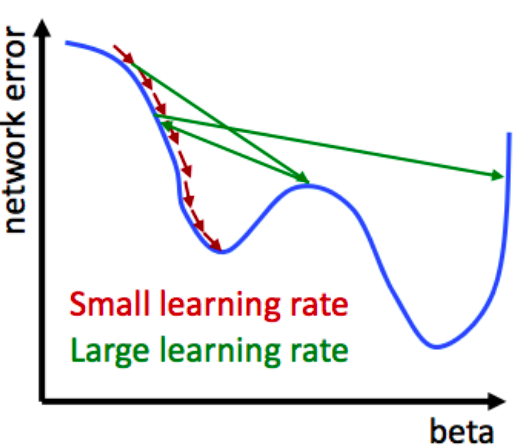
\includegraphics[width=\linewidth]{pics/learning_rate.png}
    \caption{\label{fig:bp} Learning Rate. Source: Business Analytics and Data Science Course by Professor S. Lessmann, Chapter 5: Artificial Neural Networks}
\end{figure}

Below is the code for weight's update procedure with learning rate included.

\begin{lstlisting}[language=Python]
    # Define the learning rate:
    l_r = 0.3

    # Update the weights for the links between the hidden and output layers:
    w_h_o += l_r * np.dot((o_errors * o_output * (1.0 - o_output)), np.transpose(h_output))
    # Update the weights for the links between the input and hidden layers:
    w_i_h += l_r * np.dot((h_errors * h_output * (1.0 - h_output)), np.transpose(input))
\end{lstlisting}

\subsection{Training}

So far we have been working with one particular observation. Let's put all the steps done before in a for-loop, so that we can perform them for all observations in our training set. More observations will allow the NN to learn from more information. Every time a new observation is feedforwarded, the error term backpropagated and the cost function minimized, the matrices of weights become more capable to label yet unknown observations.

\begin{lstlisting}[language=Python]
    for i in data:
        observation = i.split(',')
        input = np.array((np.asfarray(observation[1:])/255.0*0.99) + 0.01, ndmin=2).T
        target = np.array(np.zeros(o_n) + 0.01, ndmin=2).T
        target[int(observation[0])] = 0.99
    
        h_input = np.dot(w_i_h, input)
        h_output = sigmoid(h_input)
        o_input = np.dot(w_h_o, h_output)
        o_output = sigmoid(o_input)
    
        o_errors = target - o_output
        h_errors = np.dot(w_h_o.T, o_errors)
        
        w_h_o += l_r * np.dot((o_errors * o_output * (1.0 - o_output)), np.transpose(h_output))
        w_i_h += l_r * np.dot((h_errors * h_output * (1.0 - h_output)), np.transpose(input))
    
        pass
\end{lstlisting}

\subsection{Second evaluation of the results}
   
Once we have trained the model with 100 observations we can test it with new data it has never seen. After loading the test set we can first work with a particular observation to get an intuition about how good our NN can solve considered classification problem.

\begin{lstlisting}[language=Python]
    # Load the mnist test data CSV file:
    raw_data_test = open(\"data/mnist_test.csv\", 'r')
    data_test = raw_data_test.readlines()
    raw_data_test.close()
\end{lstlisting}

\begin{lstlisting}[language=Python]
    # Check a particular observation:
    observation = data_test[0].split(',')
    # Print the label:
    print(observation[0])
    # Image the number:
    image = np.asfarray(observation[1:]).reshape((28,28))
    mpp.imshow(image, cmap='Blues', interpolation='None')
\end{lstlisting}

\begin{lstlisting}
    7
\end{lstlisting}

\begin{figure}[H]
   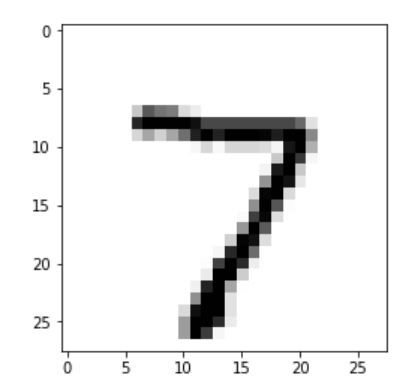
\includegraphics[width=\linewidth]{pics/7.png}
   \caption{\label{fig:number7} Plot of the handwritten number}
\end{figure}

\begin{lstlisting}[language=Python]
    # Use this observation as an input and run NN with it:
    input = np.array((np.asfarray(observation[1:])/255.0*0.99) + 0.01, ndmin=2).T
    h_input = np.dot(w_i_h, input)
    h_output = sigmoid(h_input)
    o_input = np.dot(w_h_o, h_output)
    o_output = sigmoid(o_input)
    
    o_output
\end{lstlisting}

\begin{lstlisting}
   array([[ 0.05086044],
          [ 0.01692228],
          [ 0.03306648],
          [ 0.01855151],
          [ 0.17733202],
          [ 0.01942656],
          [ 0.01083799],
          [ 0.33279056],
          [ 0.13214786],
          [ 0.05988345]])
\end{lstlisting}

\begin{lstlisting}[language=Python]
    # Get the prediction of NN for this test observation:
    label = np.argmax(o_output)
    label
\end{lstlisting}

\begin{lstlisting}
    7
\end{lstlisting}

After working with a particular observation from the test set we can label all of them and evaluate the accuracy of our NN.

\begin{lstlisting}[language=Python]   
    # Test the neural network using all test dataset:
    
    score = [] # create a list in which the predictions of the network will we saved.
    
    # Go through all the observations in the test data set:
    for i in data_test:
        observation = i.split(',')
        expected = int(observation[0])
        input = np.array((np.asfarray(observation[1:])/255.0*0.99) + 0.01, ndmin=2).T
    
        h_input = np.dot(w_i_h, input)
        h_output = sigmoid(h_input)
        o_input = np.dot(w_h_o, h_output)
        o_output = sigmoid(o_input)
    
        label = np.argmax(o_output)
    
        if (label == expected):
            score.append(1)
        else:
            score.append(0)
            pass
        
        pass
\end{lstlisting}

\begin{lstlisting}[language=Python]   
    # Calculate the performance score, the fraction of correct answers:
    score_array = np.asarray(score)
    print ("performance = ", score_array.sum() / score_array.size)
    \end{lstlisting}

\begin{lstlisting}
    performance =  0.3959
\end{lstlisting}

  It is several times better than naive, which would be 0.1 (given that we have 10 levels of the categorical variable we have to classify). Can we do better?
  
\subsection{Further Improvements}

\subsubsection{Training with several epochs}
   
One way to improve the results of the NN is to train it more. For instance we can feedforward the same 100 observations more than once. Despite the fact that these are the same observations, longer training allows NN to accumulate more knowledge. Keep in mind that due to the presence of a learning rate NN receives only part of the information that is available and useful to predict particular observation. Seeing the same observations several times leads to smaller loss of the data.
   
So let's introduce one extra parameter called epochs and create a loop around the number of epochs. The rest of the code we see below is the same as before.
   
\begin{lstlisting}[language=Python]   
    epochs = 5
\end{lstlisting}

\begin{lstlisting}[language=Python]   
    # The "big loop" with epochs:
    for e in range(epochs):
        for i in data:
            observation = i.split(',')
            input = np.array((np.asfarray(observation[1:])/255.0*0.99) + 0.01, ndmin=2).T
            target = np.array(np.zeros(o_n) + 0.01, ndmin=2).T
            target[int(observation[0])] = 0.99
    
            h_input = np.dot(w_i_h, input)
            h_output = sigmoid(h_input)
            o_input = np.dot(w_h_o, h_output)
            o_output = sigmoid(o_input)
    
            o_errors = target - o_output
            h_errors = np.dot(w_h_o.T, o_errors)
            w_h_o += l_r * np.dot((o_errors * o_output * (1.0 - o_output)), np.transpose(h_output))
            w_i_h += l_r * np.dot((h_errors * h_output * (1.0 - h_output)), np.transpose(input))
    
            pass
        pass
    
    
    # test
    score = []
    
    for i in data_test:
        observation = i.split(',')
        correct_label = int(observation[0])
        input = np.array((np.asfarray(observation[1:])/255.0*0.99) + 0.01, ndmin=2).T
    
        h_input = np.dot(w_i_h, input)
        h_output = sigmoid(h_input)
        o_input = np.dot(w_h_o, h_output)
        o_output = sigmoid(o_input)
    
        label = np.argmax(o_output)
        if (label == correct_label):
            score.append(1)
        else:
            score.append(0)
            pass
        
        pass
    
    
    # calculate accuracy
    score_array = np.asarray(score)
    print ("performance = ", score_array.sum() / score_array.size)
\end{lstlisting}

\begin{lstlisting}
    performance =  0.959
\end{lstlisting}


\subsubsection{Training with other Learning Rate}
   
The smaller the learning rate the more capable the network to optimize the weights in a more accurate way. At the same time one should keep in mind that small l\_r also means additional loss of information extracted from each particular observation. Hence, there should be many training observations available in order to make the trade-off between accuracy and usage of available data reasonable. Given that we have more epochs now, it is interesting to try a smaller learning rate.

\begin{lstlisting}[language=Python]   
    l_r = 0.1

    # run the "big loop" with epochs again to get measure accuracy for new settings.
\end{lstlisting}

\subsubsection{A more complicated structure}

As you may remember in the beginning we have assigned the number of nodes in the hidden layer based on some rule of thumb assumptions. Now we can test if the NN will perform better if we increase the number of hidden nodes.

\begin{lstlisting}[language=Python]   
    h_n = 150
    
    # Determine the weights for a bigger matrices
    w_i_h = np.random.normal(0.0, pow(h_n, -0.5), (h_n, i_n))
    w_h_o = np.random.normal(0.0, pow(o_n, -0.5), (o_n, h_n))
    
    # run the "big loop" with epochs again to get measure accuracy for new settings.
\end{lstlisting}

It is always possible to train neural networks where the number of neurons is larger. But, with a smaller number of neurons the neural network has much better generalization abilities. 

\textit{Overfitting.} To many nodes is one of the reasons that leads to a problem when the neural network is over trained which would mean that it will fail to recognize patterns which were never used in the training.

With a smaller number of neurons, it is more complicated to train the network to very small errors, but it may produce much better approximations for new patterns. The most common mistake made by many researchers is that in order to speed up the training process and to reduce the training errors, they use neural networks with a larger number of neurons than required. Such networks could perform poorly for new patterns not seen previously by the NN.

\subsubsection{Other training set}

One other source of improvement is providing the NN with a relatively big dataset for training. Everything that was done before was implemented with just 100 observations. Let's see if our results improve if we increase our training dataset to 60 000 observations. As we have more data now we will reduce the number of epochs and keep having low learning rate.

\begin{lstlisting}[language=Python]   
    # Load the data
    raw_data = open("data/mnist_train.csv", 'r')
    data = raw_data.readlines()
    raw_data.close()
    
    # Settings
    epochs = 2
    l_r = 0.1
    h_n = 90
    w_i_h = np.random.normal(0.0, pow(h_n, -0.5), (h_n, i_n))
    w_h_o = np.random.normal(0.0, pow(o_n, -0.5), (o_n, h_n))
    
    # run the "big loop" with epochs again to get measure accuracy for new settings.
\end{lstlisting}

The result we achieve with a big training set is already pretty impressive. In more than 90\% of cases our NN is able to solve the classification problem properly. And we should remember that it was implemented from scratch using only basic linear algebra packages. Let's see in the following section if we can do better or if we can simplify the process using specialized packages to build neural networks.